\documentclass[]{beamer}

\usepackage[utf8]{inputenc}
\usepackage[T1]{fontenc}
\usepackage[ngerman]{babel}

\usepackage{libertine}
\usepackage{graphicx}
\graphicspath{{./Abbildungen/}}
\usepackage{listings}

\usetheme{Madrid}
%%% Änderungen des Farbthemas
%\setbeamercolor{normal text}{fg=black,bg=red!50}
\setbeamercolor{block title}{fg=red}

%%% Änderungen des Schriftthemas
\usefonttheme{serif}
\setbeamerfont{frametitle}{size=\normalsize,series=\bfseries}

%%% Änderungen des Inneren Themas
\useinnertheme{rectangles}

%%% Weitere Anpassungen über Templates
\setbeamertemplate{navigation symbols}{}
\setbeamertemplate{itemize items}[triangle]


\begin{document}
\title{Meine erste Beamer-Präsentation}
\author{Ich \and Du}
\institute[DLR]{Deutsches Zentrum für Luft- und Raumfahrt e.\,V.}

\begin{frame}{}
    \titlepage
\end{frame}    

\begin{frame}{Gliederung}
    \tableofcontents
\end{frame}

\section{Einführung}    
\begin{frame}{Eine erste Folie}
\begin{block}{Definition}
Ein Beispiel für eine Definition
\end{block}
\pause
\begin{itemize}[<+-|alert@+>]
    \item Punkt 1
    \item Punkt 2
    \item Punkt 3
\end{itemize}
\end{frame}

\section{Hauptteil}
\begin{frame}<handout>[plain]{Bildbeispiel}
\begin{center}
    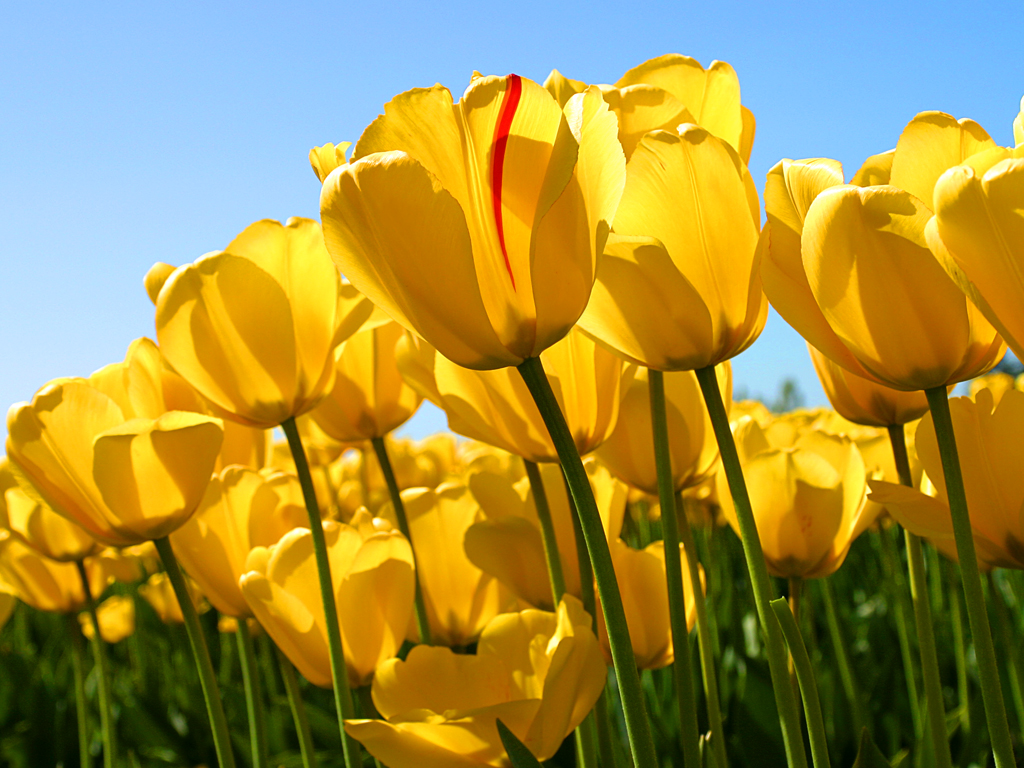
\includegraphics[width=\textwidth,height=0.8\textheight,keepaspectratio]{Tulips}
\end{center}
\end{frame}

\begin{frame}{Mach mal Pause}
Jetzt wird es spannend\pause

Ehrlich, jetzt gleich\pause

War wohl nichts
\end{frame}

\begin{frame}[fragile]{Quellcodebeispiel}
\begin{lstlisting}
\documentclass{scrbook}
\end{lstlisting}
\end{frame}


\end{document}